\documentclass[12pt]{article}
\usepackage[left=1cm, right=1cm, top=2cm,bottom=1.5cm]{geometry} 

\usepackage[parfill]{parskip}
\usepackage[utf8]{inputenc}
\usepackage[T2A]{fontenc}
\usepackage[russian]{babel}
\usepackage{enumitem}
\usepackage[normalem]{ulem}
\usepackage{amsfonts, amsmath, amsthm, amssymb, mathtools,xcolor}
\usepackage{blkarray}

\usepackage{tabularx}
\usepackage{hhline}

\usepackage{accents}
\usepackage{fancyhdr}
\pagestyle{fancy}
\renewcommand{\headrulewidth}{1.5pt}
\renewcommand{\footrulewidth}{1pt}

\usepackage{graphicx}
\usepackage[figurename=Рис.]{caption}
\usepackage{subcaption}
\usepackage{float}

%%Наименование папки откуда забирать изображения
\graphicspath{ {./images/} }

%%Изменение формата для ввода доказательства
\renewcommand{\proofname}{$\square$  \nopunct}
\renewcommand\qedsymbol{$\blacksquare$}

%%Изменение отступа на таблицах
\addto\captionsrussian{%
	\renewcommand{\proofname}{$\square$ \nopunct}%
}
%% Римские цифры
\newcommand{\RN}[1]{%
	\textup{\uppercase\expandafter{\romannumeral#1}}%
}

%% Для удобства записи
\newcommand{\MR}{\mathbb{R}}
\newcommand{\MC}{\mathbb{C}}
\newcommand{\MQ}{\mathbb{Q}}
\newcommand{\MN}{\mathbb{N}}
\newcommand{\MZ}{\mathbb{Z}}
\newcommand{\MTB}{\mathbb{T}}
\newcommand{\MTI}{\mathbb{I}}
\newcommand{\MI}{\mathrm{I}}
\newcommand{\MCI}{\mathcal{I}}
\newcommand{\MJ}{\mathrm{J}}
\newcommand{\MH}{\mathrm{H}}
\newcommand{\MT}{\mathrm{T}}
\newcommand{\MU}{\mathcal{U}}
\newcommand{\MV}{\mathcal{V}}
\newcommand{\MB}{\mathcal{B}}
\newcommand{\MF}{\mathcal{F}}
\newcommand{\MW}{\mathcal{W}}
\newcommand{\ML}{\mathcal{L}}
\newcommand{\MP}{\mathcal{P}}
\newcommand{\VN}{\varnothing}
\newcommand{\VE}{\varepsilon}

\theoremstyle{definition}
\newtheorem{defn}{Опр:}
\newtheorem{rem}{Rm:}
\newtheorem{prop}{Утв.}
\newtheorem{exrc}{Упр.}
\newtheorem{lemma}{Лемма}
\newtheorem{theorem}{Теорема}
\newtheorem{corollary}{Следствие}

\newenvironment{cusdefn}[1]
{\renewcommand\thedefn{#1}\defn}
{\enddefn}

\DeclareRobustCommand{\divby}{%
	\mathrel{\text{\vbox{\baselineskip.65ex\lineskiplimit0pt\hbox{.}\hbox{.}\hbox{.}}}}%
}
%Короткий минус
\DeclareMathSymbol{\SMN}{\mathbin}{AMSa}{"39}
%Длинная шапка
\newcommand{\overbar}[1]{\mkern 1.5mu\overline{\mkern-1.5mu#1\mkern-1.5mu}\mkern 1.5mu}
%Функция знака
\DeclareMathOperator{\sgn}{sgn}

%Функция ранга
\DeclareMathOperator{\rk}{\text{rk}}

%Обозначение константы
\DeclareMathOperator{\const}{\text{const}}

\DeclareMathOperator{\codim}{\text{codim}}

\DeclareMathOperator*{\dsum}{\displaystyle\sum}
\newcommand{\ddsum}[2]{\displaystyle\sum\limits_{#1}^{#2}}

%Интеграл в большом формате
\DeclareMathOperator{\dint}{\displaystyle\int}
\newcommand{\ddint}[2]{\displaystyle\int\limits_{#1}^{#2}}
\newcommand{\ssum}[1]{\displaystyle \sum\limits_{n=1}^{\infty}{#1}_n}

\newcommand{\smallerrel}[1]{\mathrel{\mathpalette\smallerrelaux{#1}}}
\newcommand{\smallerrelaux}[2]{\raisebox{.1ex}{\scalebox{.75}{$#1#2$}}}

\newcommand{\smallin}{\smallerrel{\in}}
\newcommand{\smallnotin}{\smallerrel{\notin}}

\newcommand*{\medcap}{\mathbin{\scalebox{1.25}{\ensuremath{\cap}}}}%
\newcommand*{\medcup}{\mathbin{\scalebox{1.25}{\ensuremath{\cup}}}}%

\makeatletter
\newcommand{\vast}{\bBigg@{3.5}}
\newcommand{\Vast}{\bBigg@{5}}
\makeatother

%Промежуточное значение для sup\inf, поскольку они имеют разную высоту
\newcommand{\newsup}{\mathop{\smash{\mathrm{sup}}}}
\newcommand{\newinf}{\mathop{\mathrm{inf}\vphantom{\mathrm{sup}}}}

%Скалярное произведение
\newcommand{\inner}[2]{\left\langle #1, #2 \right\rangle }
\newcommand{\linsp}[1]{\left\langle #1 \right\rangle }
\newcommand{\linmer}[2]{\left\langle #1 \vert #2\right\rangle }

%Подпись символов снизу
\newcommand{\ubar}[1]{\underaccent{\bar}{#1}}

%% Шапка для букв сверху
\newcommand{\wte}[1]{\widetilde{#1}}
\newcommand{\wht}[1]{\widehat{#1}}

%%Трансформация Фурье
\newcommand{\fourt}[1]{\mathcal{F}\left(#1\right)}
\newcommand{\ifourt}[1]{\mathcal{F}^{-1}\left(#1\right)}

%%Символ вектора
\newcommand{\vecm}[1]{\overrightarrow{#1\,}}

%%Пространстов матриц
\newcommand{\mat}[2]{\operatorname{Mat}_{#1, #2}}


%%Взятие в скобки, модули и норму
\newcommand{\parfit}[1]{\left( #1 \right)}
\newcommand{\modfit}[1]{\left| #1 \right|}
\newcommand{\sqparfit}[1]{\left\{ #1 \right\}}
\newcommand{\normfit}[1]{\left\| #1 \right\|}

%%Функция для обозначения равномерной сходимости по множеству
\newcommand{\uconv}[1]{\overset{#1}{\rightrightarrows}}
\newcommand{\uconvm}[2]{\overset{#1}{\underset{#2}{\rightrightarrows}}}


%%Функция для обозначения нижнего и верхнего интегралов
\def\upint{\mathchoice%
	{\mkern13mu\overline{\vphantom{\intop}\mkern7mu}\mkern-20mu}%
	{\mkern7mu\overline{\vphantom{\intop}\mkern7mu}\mkern-14mu}%
	{\mkern7mu\overline{\vphantom{\intop}\mkern7mu}\mkern-14mu}%
	{\mkern7mu\overline{\vphantom{\intop}\mkern7mu}\mkern-14mu}%
	\int}
\def\lowint{\mkern3mu\underline{\vphantom{\intop}\mkern7mu}\mkern-10mu\int}

%%След матрицы
\DeclareMathOperator*{\tr}{tr}

\makeatletter
\renewcommand*\env@matrix[1][*\c@MaxMatrixCols c]{%
	\hskip -\arraycolsep
	\let\@ifnextchar\new@ifnextchar
	\array{#1}}
\makeatother

\begin{document}
\lhead{Алгебра-\RN{1}}
\chead{Тимашев Д.А.}
\rhead{Лекция - 4}
\section*{Теорема Кронекера-Капелли}
	
Рассмотрим произвольную систему уравнений:
$$
	\left\{
	\begin{array}{ccccccccc}
		a_{11}x_1 & + & a_{12}x_2 & + & \dotsc & + & a_{1n}x_n & = & b_1 \\
		a_{21}x_1 & + & a_{22}x_2 & + & \dotsc & + & a_{2n}x_n & = & b_2 \\
		\vdots & \vdots & \vdots & \vdots & \ddots & \vdots & \vdots & \vdots & \vdots \\ 
		a_{m1}x_1 & + & a_{m2}x_2 & + & \dotsc & + & a_{mn}x_n & = & b_m 
	\end{array}
	\right.
$$
Обозначим через $A$ её матрицу коэффициентов, а через $\wte{A}$ её расширенную матрицу:
$$
	A = 
	\begin{pmatrix}
		a_{11} & \dotsc & a_{1n}\\
		\vdots & \ddots & \vdots \\
		a_{m1} & \dotsc & a_{mn}
	\end{pmatrix}, \, 
	\wte{A} = 
	\begin{pmatrix}[ccc|c]
		a_{11} & \dotsc & a_{1n} & b_1 \\
		\vdots & \ddots & \vdots  & \vdots\\
		a_{m1} & \dotsc & a_{mn} & b_m
	\end{pmatrix}
$$

\begin{theorem}(\textbf{Кронекера-Капелли})
	СЛУ совместна $\Leftrightarrow \rk{A} = \rk{\wte{A}}$.
\end{theorem}
\begin{rem}
	По-другому теорема Кронекера-Капелли может быть названа \uwave{критерием совместности}.
\end{rem}
\begin{theorem}(\textbf{критерий определенности})
	СЛУ определена $\Leftrightarrow \rk{A} = \rk{\wte{A}} = n$, где $n$ - число неизвестных.
\end{theorem}
\begin{proof}
	\hfill\\
	(\textbf{$\RN{1}$-ый способ}) Приведем матрицу $\wte{A}$ ЭП строк к ступенчатому виду $\wte{A}^*$. По методу Гаусса мы знаем, что система совместна $\Leftrightarrow r_e(A^*) = r_e\left(\wte{A}^*\right)$ и там же, система определена $\Leftrightarrow r_e(A^*) = r_e\left(\wte{A}^*\right) = n$. По теореме о совпадении трёх видов рангов матрицы мы можем утверждать:
	$$
		r_e(A^*) = \rk{A} \wedge r_e\left(\wte{A}^*\right) = \rk{\wte{A}}
	$$
	
	(\textbf{$\RN{2}$-ый способ}) Набор чисел $(\lambda_1, \dotsc, \lambda_n)$ - решение СЛУ $\Leftrightarrow \lambda_1 A^{(1)} + \dotsc + \lambda_n A^{(n)} = b$, где $b$ - столбец свободных членов.
	
	\textbf{Критерий совместности}: 
	
	$(\Rightarrow)$ пусть у СЛУ существует решение $\Leftrightarrow$ вектор-столбец $b$ линейно выражается через $\left\{A^{(1)},\dotsc, A^{(n)}\right\} \Leftrightarrow \left\{A^{(1)},\dotsc, A^{(n)}\right\}$ и $\left\{A^{(1)},\dotsc, A^{(n)},b\right\}$ линейно эквивалентны $\Rightarrow$ у линейно эквивалентных систем ранги совпадают: 
	$$
		\rk{\left\{A^{(1)},\dotsc, A^{(n)}\right\}} = \rk{\left\{A^{(1)},\dotsc, A^{(n)},b\right\}} \Leftrightarrow \rk{A} = \rk{\wte{A}}
	$$
	
	$(\Leftarrow)$ Пусть $\rk{A} = \rk{\wte{A}}$, тогда базис $\left\{A^{(j_1)},\dotsc, A^{(j_r)}\right\}$ системы столбцов $A$ является базисом и для $\wte{A}$, иначе ранг был бы больше $\Rightarrow b$ линейно выражается через $\left\{A^{(j_1)},\dotsc, A^{(j_r)}\right\} \Rightarrow$ тем более линейно выражается через все столбцы $\left\{A^{(1)},\dotsc, A^{(n)}\right\} \Rightarrow$ есть решение.
	
	\textbf{Критерий определенности}: Будем считать нашу СЛУ совместной. Тогда $\rk{A} = \rk{\wte{A}}$ и существует линейное выражение столбца $b  =\lambda_1 A^{(1)} + \dotsc + \lambda_n A^{(n)}$. Следовательно, $\rk{A} = \rk{\wte{A}} = n \Leftrightarrow$ все столбцы матрицы коэффициентов $\left\{A^{(1)},\dotsc, A^{(n)}\right\}$ линейно независимы $\Rightarrow b$ выражается через  $\left\{A^{(1)},\dotsc, A^{(n)}\right\}$ единственным способом $\Rightarrow$ существует единственное решение СЛУ $\Rightarrow$ она определена.
	
	Пусть $\rk{A} = \rk{\wte{A}} < n \Leftrightarrow \exists \, \mu_i \neq 0 \colon \mu_1 A^{(1)} + \dotsc  + \mu_n A^{(n)} = 0 \Rightarrow b = (\mu_1 + \lambda_1) A^{(1)} + \dotsc + (\mu_n + \lambda_n )A^{(n)}$ - другое линейное выражение $b \Rightarrow$ есть больше одного решения СЛУ $\Rightarrow$ система неопределена.  
\end{proof}

\newpage

\section*{Подпространства векторных пространств}

Пусть $V$ - векторное пространство. 

\begin{defn}
	\uwave{Подпространством} пространства $V$ называется непустое подмножество: $U \subseteq V, \, U \neq \VN$ для которого выполнены два свойства:
	\begin{enumerate}[label=\arabic*)]
		\item $\forall x,y \in U, \, x + y \in U$;
		\item $\forall x \in U, \, \forall \lambda \in \MR, \, \lambda{\cdot}x \in U$;
	\end{enumerate}
	То есть подпространство это непустое подмножество, замкнутое относительно операций, которые мы умеем производить над векторами.
\end{defn}
\begin{defn}
	Подпространства $U = \{0\}, \, U = V$ называются \uwave{несобственными}. Все остальные подпространства - \uwave{собственные}.
\end{defn}

\subsection*{Свойства подпространств}

\begin{prop}
	$\vecm{0} \in U$.
\end{prop}
\begin{proof}
	В самом деле, $U \neq \VN \Rightarrow \exists \, x \in U \Rightarrow 0{\cdot}x  = \vecm{0} \in U$.
\end{proof}

\begin{prop}
	$U$ само является векторным пространством и операции на множестве $U$ получаются ограничением операций на $V$.
\end{prop}
\begin{proof}
	Операции не выходят за множество $U$ по определению, аксиомы выполняются также автоматически, поскольку они выполняются на большем множестве $V$.
\end{proof}

\subsection*{Примеры: геометрическое пространство}

$V = \{\text{геом. векторы в пространстве}\}, \, U = \{\text{геом. векторы на заданной плоскости в пространстве}\}$.
\begin{figure}[H]
	\centering
	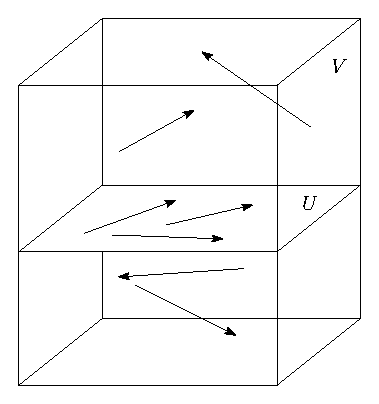
\includegraphics[width=0.3\textwidth]{AL4_1.eps}
	\caption{Геометрические векторы в плоскости $U$ пространства $V$.}
	\label{4_1}
\end{figure}
\begin{proof}
	Сумма двух векторов в плоскости снова будет лежать в плоскости, при умножении вектора на число мы не выходим за пределы этой плоскости, поэтому это будет подпространством.
\end{proof}
\newpage

\subsection*{Примеры: линейные оболочки}
Пусть $S \subseteq V$ - система векторов.

\begin{defn}
	\uwave{Линейной оболочкой} $S$ назовём множество всех линейных комбинаций векторов из $S$: 
	$$
		U = \linsp{S} = \{v = \lambda_1 v_1 + \dotsc + \lambda_m v_m \mid v_i \in S, \, \lambda_i \in \MR\}
	$$
\end{defn}
\begin{proof}\hfill\\
	Если $S = \VN \Rightarrow \linsp{S} = \left\{\vecm{0}\right\} \neq \VN$. Сумма в которой нет слагаемых по определению равна $0$.
	
	Если $S \neq \VN \Rightarrow \forall v_1, \dotsc, v_m \in S, \, 0{\cdot}v_1 + \dotsc + 0{\cdot}v_m = \vecm{0} \in \linsp{S} \Rightarrow \linsp{S} \neq \VN$. 
	
	\begin{enumerate}[label=\arabic*)]
		\item $\forall x,y \in \linsp{S}, \, x + y = \lambda_1 v_1 + \dotsc + \lambda_m v_m + \mu_1 v_1 + \dotsc + \mu_m v_m = (\lambda_1 + \mu_1)v_1 + \dotsc + (\lambda_m + \mu_m)v_m \in \linsp{S}$;
		\item $\forall x \in \linsp{S}, \, \forall \lambda \in \MR, \, \lambda{\cdot}x = \lambda{\cdot}\mu_1 v_1 + \dotsc + \lambda{\cdot}\mu_m v_m = (\lambda {\cdot} \mu_1) v_1 + \dotsc + (\lambda {\cdot} \mu_m)v_m \in \linsp{S}$;
	\end{enumerate}
\end{proof}
\begin{defn}
	Если $U = \linsp{S}$, то говорят, что подмножество $S$ \uwave{порождает} подпространство $U$.
\end{defn}
\begin{rem}
	Заметим, что это наименьшее подпространство, содержащее $S$, поскольку если множество $S$ лежит в каком-то подпространстве, то там же лежат и все линейные комбинации векторов из $S$.
\end{rem}
\begin{rem}
	Также заметим, что линейная оболочка вссегда бесконечна, кроме того случая, когда является линейной оболочкой $0$. В остальных случаях вместе с любым вектором она содержит и всю прямую.
\end{rem}
\begin{prop}
	Если $B$ - это базис в $S$, то $B$ и базис в $\linsp{S}$.
\end{prop}
\begin{proof}
	Пусть $B = \{e_1, \dotsc, e_n\}$, тогда $\forall v \in S, \, v = \lambda_1 e_1 + \dotsc + \lambda_n e_n, \, \lambda_ i \in \MR, \, i =\overline{1,n}$. Тогда:
	$$
		\forall w \in \linsp{S}, \, w = \mu_1 v_1 + \dotsc + \mu_m v_m, \, v_i = \ddsum{j = 1}{n}\alpha_{ij}e_j \in S, \, i = \overline{1,m}, \, \alpha_{ij} \in \MR, \, \forall i,j \Rightarrow 
	$$
	$$
		\Rightarrow w = \ddsum{i = 1}{m}\ddsum{j = 1}{n}\mu_i\alpha_{ij}e_j = \ddsum{j = 1}{n} \ddsum{i = 1}{m} \mu_i\alpha_{ij}e_j =  w_1 e_1 + \dotsc + w_n e_n, \, w_j \in \MR, \, \forall j = \overline{1,n}
	$$ 
\end{proof}
\begin{corollary}
	$\dim{\linsp{S}} = \rk{S}$.
\end{corollary}
\begin{proof}
	Поскольку базисы у $S$ и $\linsp{S}$ одинаковые, то число векторов в них также одинаково.
\end{proof}

\begin{prop}
	Любое подпространство $U$ является линейной оболочкой своего базиса $B = \{e_1, \dotsc, e_m\}$.
\end{prop}
\begin{proof}
	Базис по определению обладает тем свойством, что любой вектор из подпространства является линейной комбинацией векторов из базиса: 
	$$
		\forall u \in U, \, u =\mu_1 e_1 + \dotsc + \lambda_m e_m, \, \mu_i \in \MR, \, i = \overline{1,m}
	$$
	Взяв все линейные комбинации базисных векторов мы получим все векторы из этого подпространства:
	$$
		U = \{u = \lambda_1 e_1 + \dotsc + \lambda_m e_m \mid e_i \in B, \, \lambda_i \in \MR \} = \linsp{\{e_1 ,\dotsc, e_m\}} = \linsp{B}
	$$
\end{proof}

\newpage
\section*{Фундаментальная система решений}
Подпространства в арифметическом пространстве (а значит и в любом конечномерном пространстве) также можно задавать с помощью ОСЛУ.
\begin{theorem}
	Рассмотрим произвольную ОСЛУ с матрицей коэффициентов $A$:
	$$
		\left\{
		\begin{array}{ccccccc}
			a_{11}x_1 & + & \dotsc & + & a_{1n}x_n & = &  0\\
			\vdots  & \vdots & \ddots & \vdots & \vdots & \vdots & \vdots \\ 
			a_{m1}x_1 &  + & \dotsc & + & a_{mn}x_n & = & 0 
		\end{array}
		\right.
	$$
	Тогда множество её решений: $U \subseteq \MR^n$ будет подпространством и $\dim{U} = n - \rk{A}$. 
\end{theorem}
\begin{proof}
	Докажем, что $U$ - подпространство. 
	
	Множество решений всегда содержит нулевой вектор: $(0, \dotsc, 0) \in U \Rightarrow U \neq \VN$.
	\begin{enumerate}[label=\arabic*)]
		\item Пусть $y = (y_1, \dotsc, y_n), \, z = (z_1, \dotsc, z_n) \in U$, тогда будет верно:
		$$
			\forall i = \overline{1,m}, \, a_{i1}y_1 + \dotsc + a_{in} y_n = 0, \, a_{i1}z_1 + \dotsc + a_{in} z_n = 0 \Rightarrow 
		$$
		$$
			\Rightarrow a_{i1}(y_1 + z_1)  + \dotsc + a_{in} (y_n + z_n) = 0 \Rightarrow y + z = (y_1 + z_1, \dotsc , y_n  + z_n) \in U
		$$
		\item Пусть $y = (y_1, \dotsc, y_n) \in U, \, \lambda \in \MR$, тогда будет верно:
		$$
			\forall i = \overline{1,m}, \, a_{i1}y_1 + \dotsc + a_{in} y_n = 0 \Rightarrow \lambda{\cdot}(a_{i1}y_1 + \dotsc + a_{in} y_n) = a_{i1}{\cdot} \lambda y_1 + \dotsc + a_{in} {\cdot} \lambda y_n = 0 \Rightarrow 
		$$
		$$
			\Rightarrow a_{i1}(\lambda y_1) + \dotsc + a_{in}(\lambda y_n) = 0 \Rightarrow\lambda {\cdot}y = (\lambda y_1 ,\dotsc, \lambda y_n) \in U 
		$$
	\end{enumerate}
	Найдем базис подпространства $U \Rightarrow$ построим его (поскольку во всех базисах одинаковое число векторов, то нам не важно какой это будет базис). Воспользуемся методом Гаусса и приведем ОСЛУ к ступенчатому виду $\Rightarrow$ возникают главные неизвестные: $x_{j_1}, \dotsc, x_{j_r}$ и свободные неизвестные: $x_j, \, j \neq j_1,\dotsc, j_r$. Следовательно, мы получаем общее решение - выражение главных неизвестных через свободные:
	$$
		\forall k = \overline{1,r}, \, x_{j_k} = \ddsum{j \neq j_1, \dotsc, j_r}{}c_{kj}x_j
	$$
	Поскольку наша система однородна, то в выражении выше не будет свободного члена. Подставляя вместо свободных неизвестных конкретные числовые значения, мы будем получать частные решения. 	
	Построим частное решение $v_j, \, \forall j \neq j_1,\dotsc,j_r$ следующим образом:
	$$
		x_j = 1, \, x_i = 0, \, \forall i \neq j_1, \dotsc, j_r, j \Rightarrow x_{j_k} = c_{kj}
	$$ 
	Запишем это в векторной форме:
	$$
		v_j = (0, \dotsc, \underset{j_1}{c_{1j}},  \dotsc,0, \underset{j}{1}, 0, \dotsc, \underset{j_r}{c_{rj}}, \dotsc, 0)
	$$
	Таких векторов у нас будет столько же, сколько и номеров свободных неизвестных, то есть  $n - r$. Докажем, что их множество $\{v_j \mid j \neq j_1 ,\dotsc, j_r\}$ и будет искомым базисом $U$.
	
	\uline{\textbf{Линейная независимость}}: Пусть произвольная линейная комбинация равна нулю:
	$$
		\ddsum{j \neq j_1, \dotsc, j_r}{}\lambda_j v_j = 0 \Rightarrow \forall j \neq j_1, \dotsc, j_r,\, \ddsum{j \neq j_1, \dotsc, j_r}{}\lambda_j v_j = \lambda_j {\cdot}1 + \ddsum{i \neq j, j_1,\dotsc, j_r}{}\lambda_{i}{\cdot}0 = \lambda_j = 0
	$$
	
	\uline{\textbf{Порождает}} $U$: Для любого решения $z = (z_1, \dotsc, z_n) \in U$ рассмотрим новый вектор $z'$, который является линейной комбинацией векторов $v_j$ с коэффициентами, которые равны соответствующим координатам вектора $z$: 
	$$
		z' = \ddsum{j \neq j_1, \dotsc, j_r}{}z_jv_j
	$$
	По доказанному ранее, $z'_j = z_j, \, \forall j \neq j_1, \dotsc, j_r \Rightarrow$ координаты свободных неизвестных совпадают $\Rightarrow$ координаты главных неизвестных также будут совпадать, поскольку они однозначно выражаются через свободные из общего решения $\Rightarrow z'_{j_k} = z_{j_k}, \, \forall k = 1,\dotsc,r \Rightarrow z = z'$. Следовательно, любое решение выражается в виде комбинации $v_j$.
	
	Таким образом, мы доказали, что $\{v_j \mid j \neq j_1 ,\dotsc, j_r\}$ - базис $\Rightarrow \dim{U} = n -r = n - r_e(A^*)$, поскольку число главных неизвестных равно числу ненулевых строк в ступенчатой матрице. Следовательно:
	$$
		\dim{U} = n - r_e(A^*) = n - \rk{A}
	$$
\end{proof}

\begin{defn}
	Базис пространства $U$ решений ОСЛУ называется \uwave{фундаментальной системой решений} (ФСР). 
\end{defn}

\section*{Неоднородная система линейных уравнений}
Рассмотрим произвольную СЛУ:
$$
	\left\{
	\begin{array}{ccccccc}
		a_{11}x_1 & + & \dotsc & + & a_{1n}x_n & = &  b_1\\
		\vdots  & \vdots & \ddots & \vdots & \vdots & \vdots & \vdots \\ 
		a_{m1}x_1 &  + & \dotsc & + & a_{mn}x_n & = & b_m
	\end{array}
	\right.
$$
И свяжем с этой системой ОСЛУ, заменив свободные члены на нули:
$$
	\left\{
	\begin{array}{ccccccc}
		a_{11}x_1 & + & \dotsc & + & a_{1n}x_n & = & 0\\
		\vdots  & \vdots & \ddots & \vdots & \vdots & \vdots & \vdots \\ 
		a_{m1}x_1 &  + & \dotsc & + & a_{mn}x_n & = & 0
	\end{array}
	\right.
$$
\begin{defn}
	Связанная с произвольной СЛУ однородная СЛУ называется \uwave{ассоциированной}.
\end{defn}
\begin{defn}
	\uwave{Линейным многообразием} в пространстве $\MR^n$ называется подмножество $L \subseteq \MR^n$ для которого $\exists \, v \in \MR^n$ и $\exists \, U \subseteq \MR^n$ такие, что:
	$$
		L = v + U = \{y \in \MR^n \mid y = v + z, \, z \in U\}
	$$ 
\end{defn}
\begin{rem}
	То есть, линейное многообразие это по сути сдвиг подпространства на какой-то вектор, вообще говоря в этом подпространстве не лежащий.
\end{rem}
\begin{prop}
	Пусть СЛУ совместна, $U \subseteq \MR^n$ - пространство решений ассоциированной однородной СЛУ и $x^{\circ} = (x^{\circ}_1, \dotsc, x^{\circ}_n) \in \MR^n$ - её частное решение. Тогда множество всех решений СЛУ имеет вид: 
	$$
		x^{\circ} + U = \{y \in \MR^n \mid y = x^{\circ} + z, \, z \in U\}
	$$
	То есть множество решений неоднородной СЛУ является линейным многообразием.
\end{prop}
\begin{proof}
	Надо показать, что два множества совпадают $\Rightarrow$ покажем, что каждое решение СЛУ имеет вид $x^{\circ} + z, \, z \in U$ и наобоорт, что каждый вектор такого вида является решением.
	
	$(\Rightarrow)$ Пусть $y$ - решение СЛУ $\Rightarrow \forall i = \overline{1,m},\, a_{i1}y_1 +  \dotsc + a_{in}y_n = b_i$, вместе с этим $x^{\circ}$ - тоже решение СЛУ, тогда: $\forall i = \overline{1,m},\, a_{i1}x^{\circ}_1 +  \dotsc + a_{in}x^{\circ}_n = b_i \Rightarrow$ вычтем одно решение из другого:
	$$
		a_{i1}(y_1 - x^{\circ}_1) + a_{i2}(y_2 - x^{\circ}_2) + \dotsc + a_{in}(y_n - x^{\circ}_n) = 0
	$$
	Следовательно, вектор $z = y - x^{\circ} \in U \Rightarrow y = x^{\circ} + z$.
	
	$(\Leftarrow)$ Если $z \in U \Rightarrow \forall i = \overline{1,m}, \, a_{i1}z_1 + \dotsc + a_{in}z_n = 0$. Сложим это равенство с равенствами при частном решении на $x^{\circ}$:
	$$
		\forall i = \overline{1,m}, \, a_{i1}(x_1^{\circ} + z_1 ) + \dotsc + a_{in}(x_n^{\circ} + z_n) = b_i
	$$
	Таким образом, $y = x^{\circ} + z$, где $z \in U$ - произвольное, тоже будет решением исходной СЛУ.
\end{proof}
\begin{figure}[H]
	\centering
	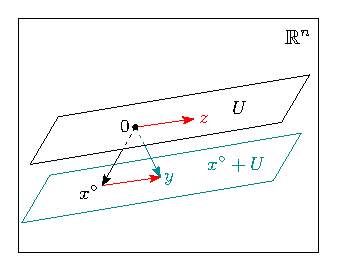
\includegraphics[width=0.4\textwidth]{AL4_2.eps}
	\caption{Геометрическое устройство множества решений произвольной неоднородной СЛУ.}
	\label{4_2}
\end{figure}

\subsection*{Пример}
Пусть $n = 3$, рассмотрим следующую СЛУ:
$$
	\left\{
		x_1 +2x_2 + 4x_3 = 8
	\right.
$$
Её ассоциированная ОСЛУ будет иметь вид:
$$
	\left\{
		x_1 +2x_2 + 4x_3 = 0
	\right.
$$
Система уже приведена к ступенчатому виду, тогда:
\begin{enumerate}[label=\arabic*)]
	\item \textbf{\uline{главные неизвестные}}: $x_1$;
	\item \textbf{\uline{свободные неизвестные}}: $x_2,x_3$;
	\item \textbf{\uline{общее решение ОСЛУ}}: $x_1 = - 2x_2 - 4x_3$;
	\item \textbf{\uline{общее решение СЛУ}}: $x_1 = 8 - 2x_2 - 4x_3$;
\end{enumerate}
Обозначим $U \subseteq \MR^3$ - пространство решений ОСЛУ, $\dim{U} = 3- 1 = 2$. Получим ФСР, подставляя вместо какой-то свободной неизвестной $1$, а остальным придаем значения $0$ и находим значения главных неизвестных, тогда: 
$$
	v_2 = (-2,1,0), \, v_3 =  (-4,0,1)
$$
\begin{rem}
	Фундаментальне решения нумеруются номерами тех свободных неизвестных, которым мы придаем значения $1$.
\end{rem}
Для описания линейного многообразия нам необходимо найти ещё какое-нибудь частное решение. Пусть все свободные неизвестные равны $0$, тогда частное решение СЛУ будет иметь вид:
$$
	x^{\circ} = (8,0,0)
$$
Изобразим графически множество решений. Выберем в пространстве координатные оси и будем по ним откладывать координаты: $(x_1, x_2, x_3)$. Тогда каждый вектор в этом геометрическом пространстве имеет три координаты и его можно отождествить с арифметическим вектором (с тройкой из этих координат). Пространство решений ОСЛУ будет двумерным $\Rightarrow$ плоскостью.

Пересечение полученного множества с координатными осями будет в точках: $(8, 0,0),\, (0,4,0), \, (0,0,2)$. То есть множество решений нашей СЛУ из одного линейного уравнения это плоскость, содержащая треугольник построенный пунктирными линиями на графике.
\begin{figure}[H]
	\centering
	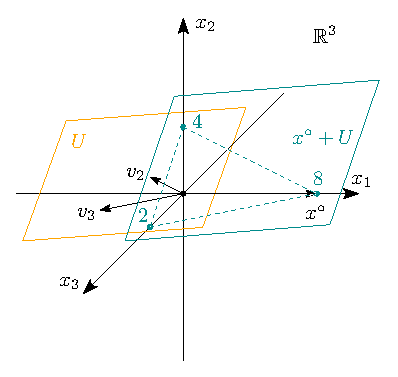
\includegraphics[width=0.55\textwidth]{AL4_3.eps}
	\caption{Построение множества решений СЛУ.}
	\label{4_3}
\end{figure}
\newpage
Отметим, что можно двигаться и в обратную сторону и по подпространству построить СЛУ, множеством решения которой будет является это подпространство.
\begin{theorem}\hfill
	\begin{enumerate}[label=\arabic*)]
		\item Пусть $U \subset \MR^n$ - некоторое подпространство. Тогда существует ОСЛУ от переменных $x_1, \dotsc, x_n$, множество решений которой равно $U$;
		\item Пусть $L \subset \MR^n$ - линейное многообразие. Тогда существует СЛУ от $n$ неизвестных, множество решений которой равно $L$;
	\end{enumerate}
\end{theorem}

\begin{proof}
	\hfill
	\begin{enumerate}[label=\arabic*)]
		\item Пусть $\{v_1,\dotsc, v_k\}$ - базис $U$, где: $v_i = (a_{i1}, a_{i2},\dotsc,a_{in}), \, \forall i = \overline{1,k}$. Запишем СЛУ с матрицей коэффициентов $A$:
		$$
			\left\{
				\begin{array}{ccccccccc}
					a_{11}x_1 &+& a_{12}x_2 &+& \dotsc &+& a_{1n}x_n &=& 0\\
					a_{21}x_1 &+& a_{22}x_2 &+& \dotsc &+& a_{2n}x_n &=& 0\\
					\vdots &\vdots& \vdots & \vdots & \ddots &\vdots& \vdots &\vdots & \vdots\\
					a_{k1}x_1 &+& a_{k2}x_2 &+& \dotsc &+& a_{kn}x_n &=& 0
				\end{array}
			\right.
		$$
		Рассмотрим ФСР для этой системы: $\{w_1,\dotsc, w_m\}$, где $w_i = (c_{i1}, c_{i2}, \dotsc, c_{in}), \, \forall i =\overline{1,m}$. Тогда по теореме $3$ будет верно: $m = n -\rk{A}$, если $\rk{A} = k$, то $m = n - k$. Рассмотрим систему с матрицей коэффициентов $C$:
		$$
			\left\{
				\begin{array}{ccccccccc}
					c_{11}x_1 &+& c_{12}x_2 &+& \dotsc &+& c_{1n}x_n &=& 0\\
					c_{21}x_1 &+& c_{22}x_2 &+& \dotsc &+& c_{2n}x_n &=& 0\\
					\vdots &\vdots& \vdots & \vdots & \ddots &\vdots& \vdots &\vdots & \vdots\\
					c_{m1}x_1 &+& c_{m2}x_2 &+& \dotsc &+& c_{mn}x_n &=& 0
				\end{array}
			\right.
		$$
		Обозначим через $V$ подпространство решений этой системы в $\MR^n$. По построению $v_1, \dotsc, v_k$ - это решение этой системы. Следовательно, $U \subseteq V$. С другой стороны: 
		$$
			\dim{V} = n - \rk{C} = n - m
		$$
		Таким образом, мы получаем: $n - m = n - (n - k) = k = \dim{U} = \dim{V}$. А поскольку $U \subseteq V$ и $\dim{U} = \dim{V}$, тогда $U = V$;
		\item Если $L = \VN$, то система может быть экзотической:
		$$
			0{\cdot}x_1 + 0{\cdot}x_2 + \dotsc + 0{\cdot}x_n = 1
		$$
		Пусть $L \neq \VN$, тогда по определению линейного многообразия $L = v + U$, где $U \subseteq \MR^n$ - подпространство. Пусть:
		$$
			\left\{
				\begin{array}{ccccccccc}
					c_{11}x_1 &+& c_{12}x_2 &+& \dotsc &+& c_{1n}x_n &=& 0\\
					c_{21}x_1 &+& c_{22}x_2 &+& \dotsc &+& c_{2n}x_n &=& 0\\
					\vdots &\vdots& \vdots & \vdots & \ddots &\vdots& \vdots &\vdots & \vdots\\
					c_{m1}x_1 &+& c_{m2}x_2 &+& \dotsc &+& c_{mn}x_n &=& 0
				\end{array}
			\right.
		$$
		это однородная система с множеством решений $U$ (существует по первому пункту). Пусть верно:
		$$
			v = (\alpha_1, \dotsc, \alpha_n), \, b_i = c_{i1}\alpha_1 + c_{i2}\alpha_2 + \dotsc + c_{in}\alpha_n, \, \forall i = \overline{1,m}
		$$
		Тогда система:
		$$
			\left\{
				\begin{array}{ccccccccc}
					c_{11}x_1 &+& c_{12}x_2 &+& \dotsc &+& c_{1n}x_n &=& b_1\\
					c_{21}x_1 &+& c_{22}x_2 &+& \dotsc &+& c_{2n}x_n &=& b_2\\
					\vdots &\vdots& \vdots & \vdots & \ddots &\vdots& \vdots &\vdots & \vdots\\
					c_{m1}x_1 &+& c_{m2}x_2 &+& \dotsc &+& c_{mn}x_n &=& b_m
				\end{array}
			\right.
		$$
		будет СЛУ, множество решений которой равно $L$, то есть мы получили искомую СЛУ.
	\end{enumerate}
\end{proof}

\end{document}